\section{Creazione delle istanze AWS}

Creiamo il nostro account AWS al \underline{\href{https://aws.amazon.com/it/}{seguente link}} e accediamo per raggiungere la console di AWS:

\begin{figure}[H]
    \centering
    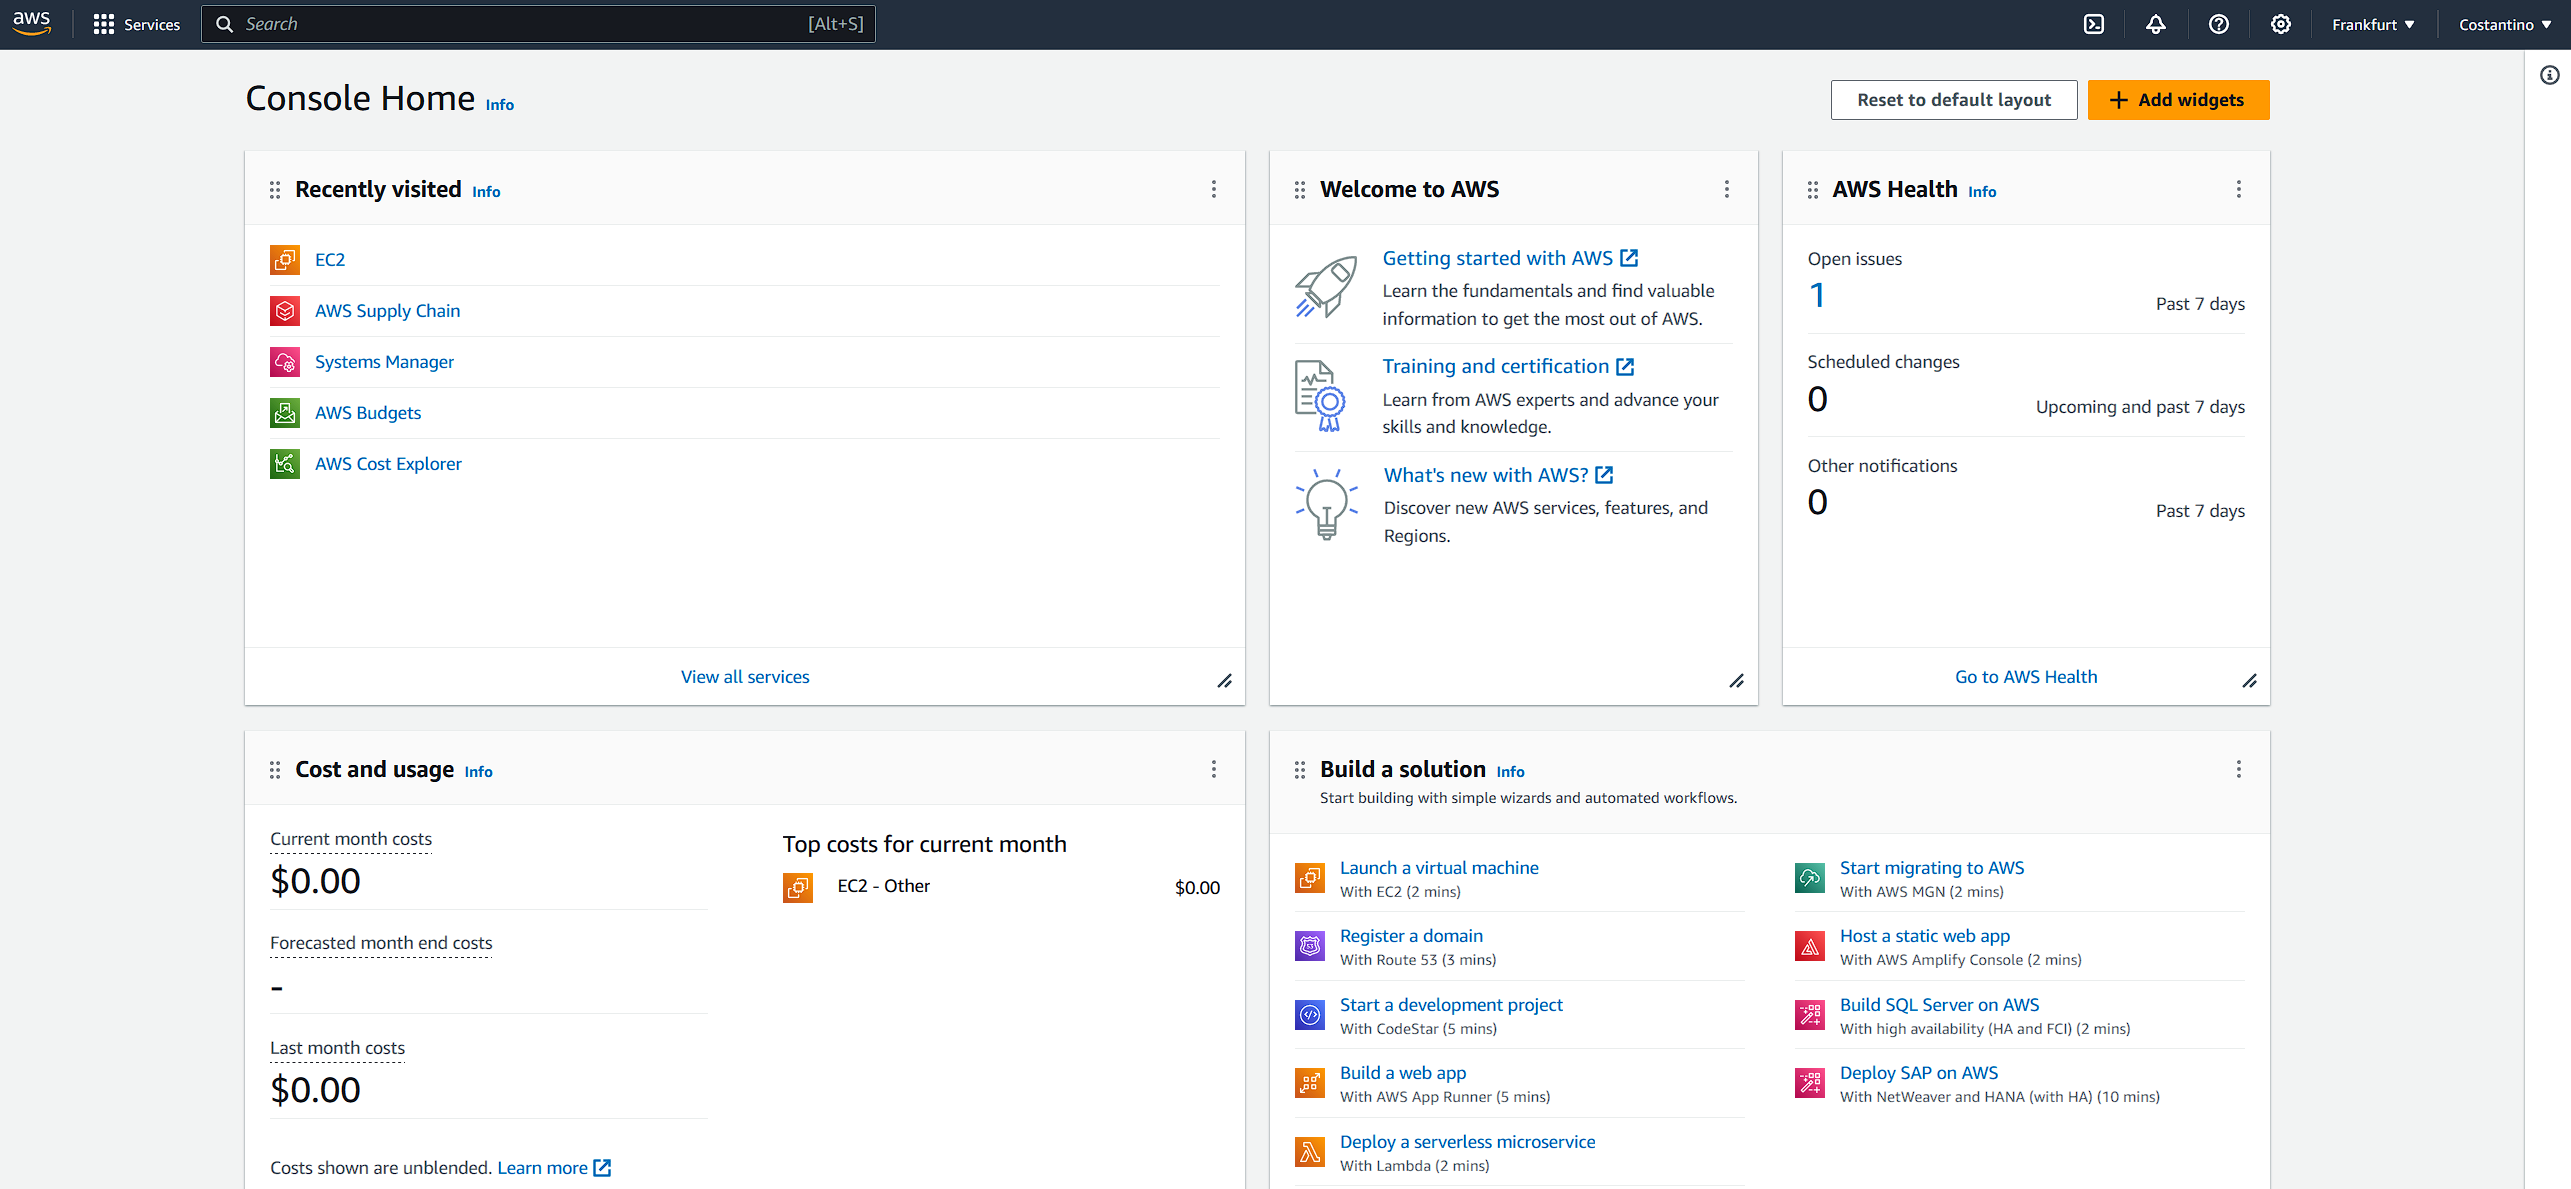
\includegraphics[width=0.95\textwidth]{images/aws-console.png}
\end{figure}

Amazon fornisce una serie di servizi. Quello che andremo a utilizzare noi è \textbf{Amazon Elastic Compute Cloud} (\textbf{Amazon EC2}), il quale offre un piano gratuito che include 750 ore mensili per l'utilizzo di istanze t2.micro Linux e Windows per un anno.

Una volta nella \textbf{dashboard di EC2} (che si può raggiungere tramite la barra di ricerca della console), selezioniamo il pulsante arancione \textbf{Launch instance}, e iniziamo così la creazione delle istanze.
Nella sezione \textbf{Application and OS Images} ci viene permesso di scegliere il tipo di sistema che vogliamo per le nostre istanze (le istanze che rientrano nel piano delle 750 ore sono quelle che riportano la scritta \textit{Free tier eligible}). Per una questione di semplicità la scelta del sistema operativo è ricaduta su \textbf{Ubuntu 22.04}:

\begin{figure}[H]
    \centering
    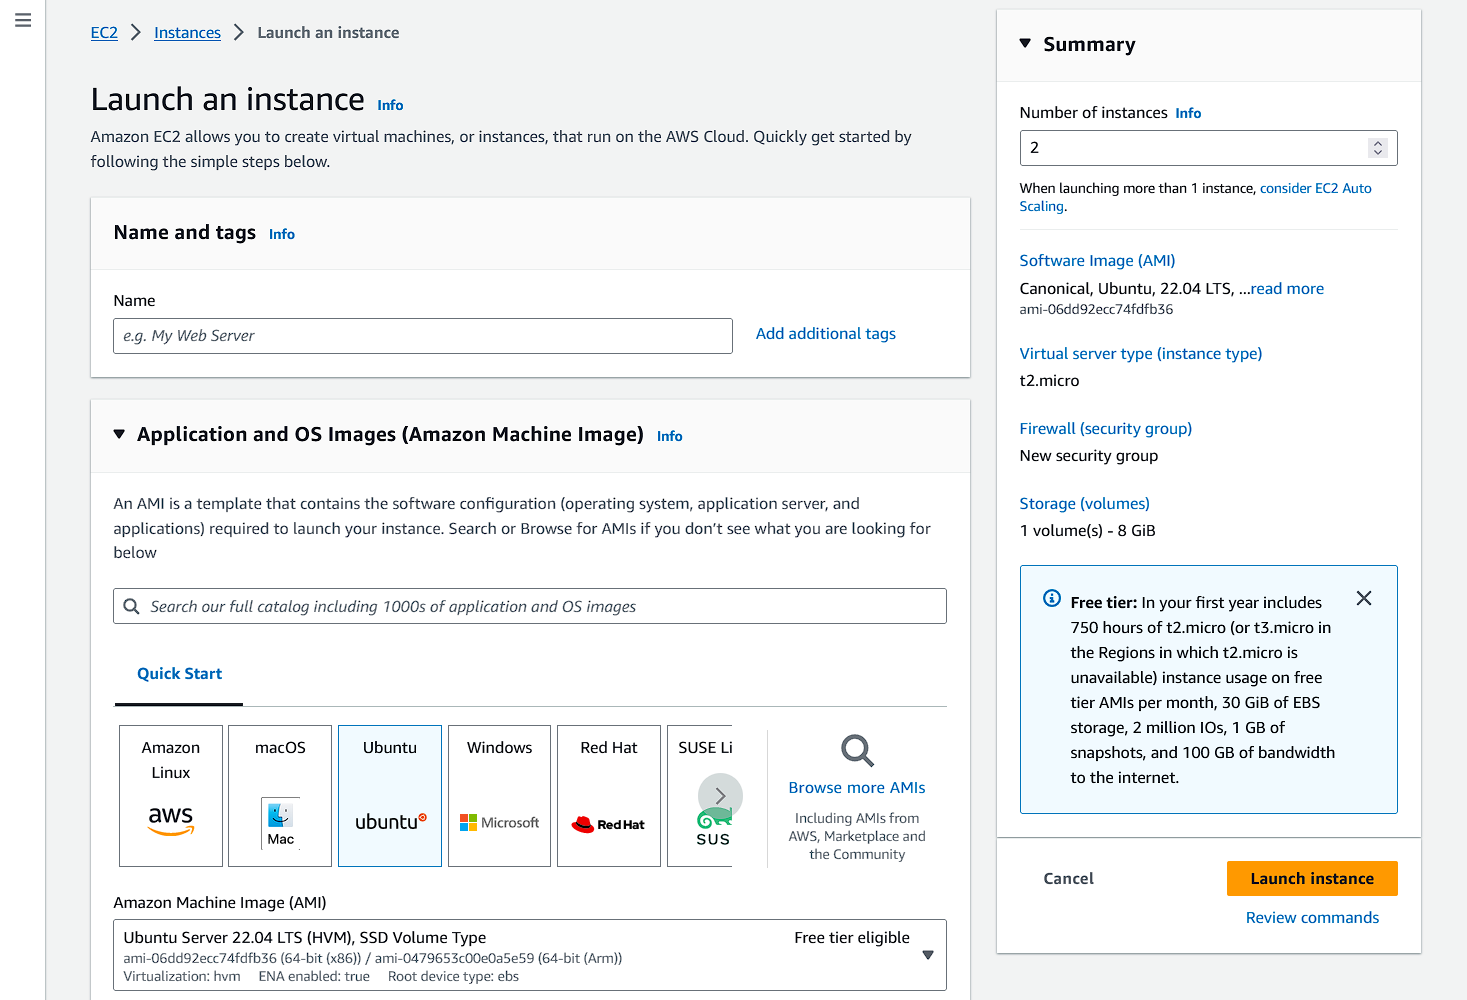
\includegraphics[width=0.8\textwidth]{images/vm-selection.png}
\end{figure}

Scelto il sistema operativo proseguiamo fino alla sezione \textbf{Instance type} e assicuriamoci che l'opzione selezionata sia \textbf{t2.micro} (l'unica \textit{Free tier eligible}):

\begin{figure}[H]
    \centering
    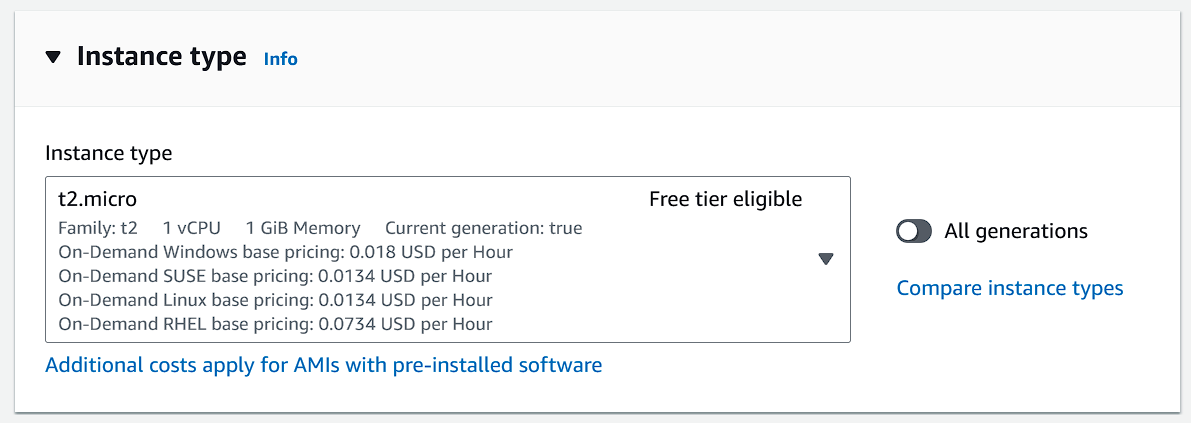
\includegraphics[width=0.65\textwidth]{images/instance-type.png}
\end{figure}

Proseguiamo da qui nella configurazione delle istanze raggiungendo la sezione \textbf{Key pair (login)} e clicchiamo su \textbf{Create a new key pair}:

\begin{figure}[H]
    \centering
    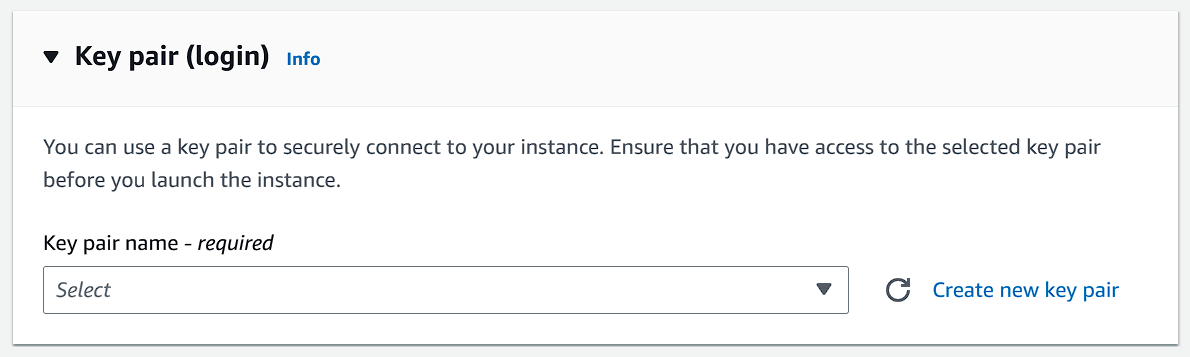
\includegraphics[width=0.65\textwidth]{images/key-pair.png}
\end{figure}

Nel popup che si aprirà impostiamo come nome \textbf{my-key}, come tipo di chiave \textbf{RSA} e come formato \textbf{.pem}:

\begin{figure}[H]
    \centering
    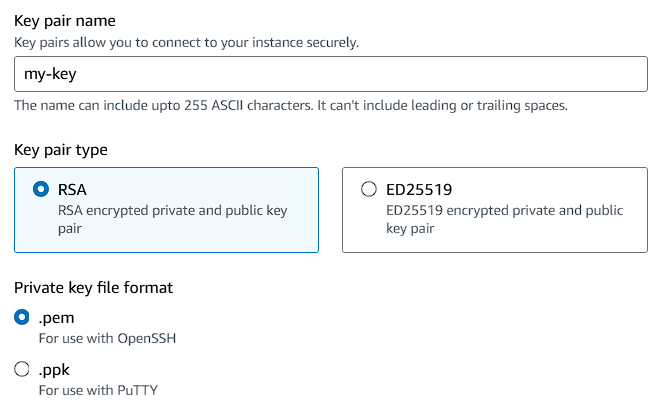
\includegraphics[width=0.65\textwidth]{images/key-creation.png}
\end{figure}

Vi verrà chiesto di salvare questa chiave sul computer. È molto importante salvarla in un posto sicuro, perché senza non è possibile accedere alle istanze da terminale (vi è la possibilità di farlo dal sito ma non è molto comodo).

Nota: se vi trovate su una distribuzione Linux o Mac dovrete settare il permesso alla chiave con il comando seguente:

\begin{verbatim}
    $ chmod 400 my-key.pem
\end{verbatim}

Raggiungiamo ora la sezione \textbf{Network settings} e clicchiamo sul pulsante \textbf{Edit} in alto a destra:

\begin{figure}[H]
    \centering
    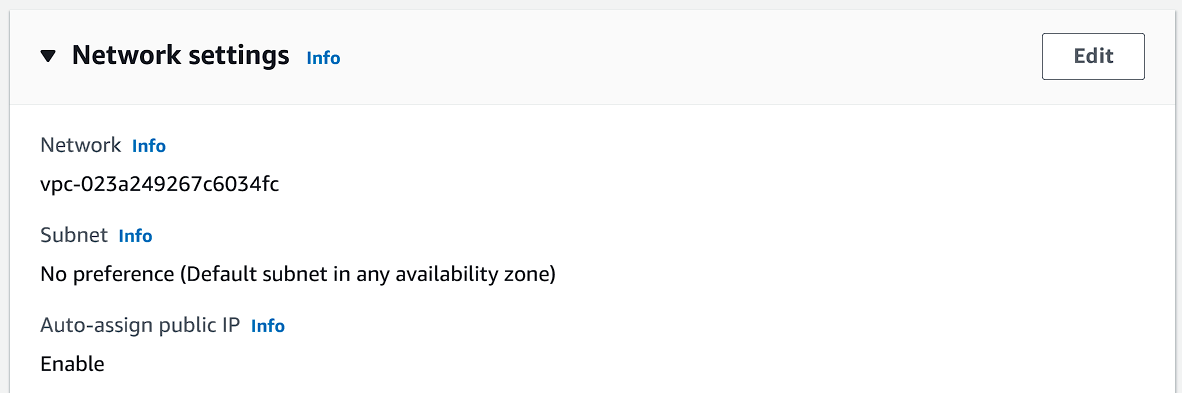
\includegraphics[width=0.65\textwidth]{images/network.png}
\end{figure}

Tramite il pulsante che apparirà in fondo alla sezione (\textbf{Add security group rule}) creiamo una seconda regola per le porte da utilizzare nelle nostre istanze. Scegliamo per il tipo l'opzione \textbf{All traffic} e per il tipo di sorgente la voce \textbf{Anywhere}. Alla fine dovremmo avere una seconda regola come appare nella seguente figura:

\begin{figure}[H]
    \centering
    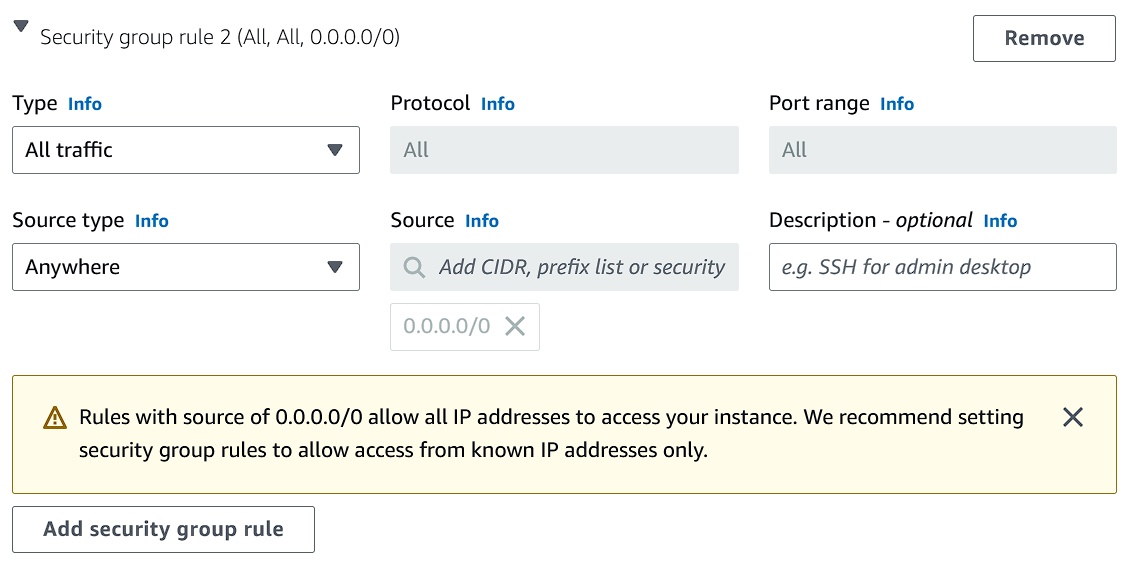
\includegraphics[width=0.65\textwidth]{images/security-rule.png}
\end{figure}

Dal sommario (in alto a destra o in fondo alla pagina, a seconda della dimensione della finestra del browser) impostiamo infine il numero di istanze a \textbf{2}, e clicchiamo sul pulsante \textbf{Launch instance} per crearle.

Verremo riportati alla schermata con l'elenco delle istanze, dove potremmo rinominare le due nuove istanze appena create. Chiamiamo l'istanza master \textbf{namenode} e quella slave \textbf{datanode2}. Fatto questo selezioniamo le istanze e avviamole dal menu a tendina del pulsante \textbf{Instance state} (se non si stanno già avviando):

\begin{figure}[H]
    \centering
    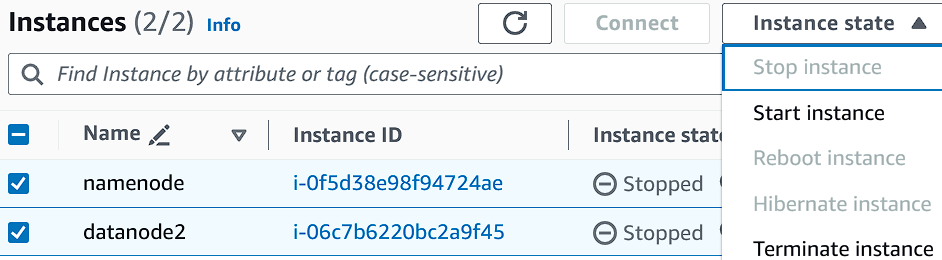
\includegraphics[width=0.7\textwidth]{images/activate-instance.png}
\end{figure}

Selezionando un'istanza alla volta e cliccando sul tasto \textbf{Connect} apparirà una schermata per la connessione. Andando nella sezione \textbf{SSH client} si può trovare il comando ssh con cui connettersi alla istanza selezionata che è possibile copiare per comodità:

\begin{figure}[H]
    \centering
    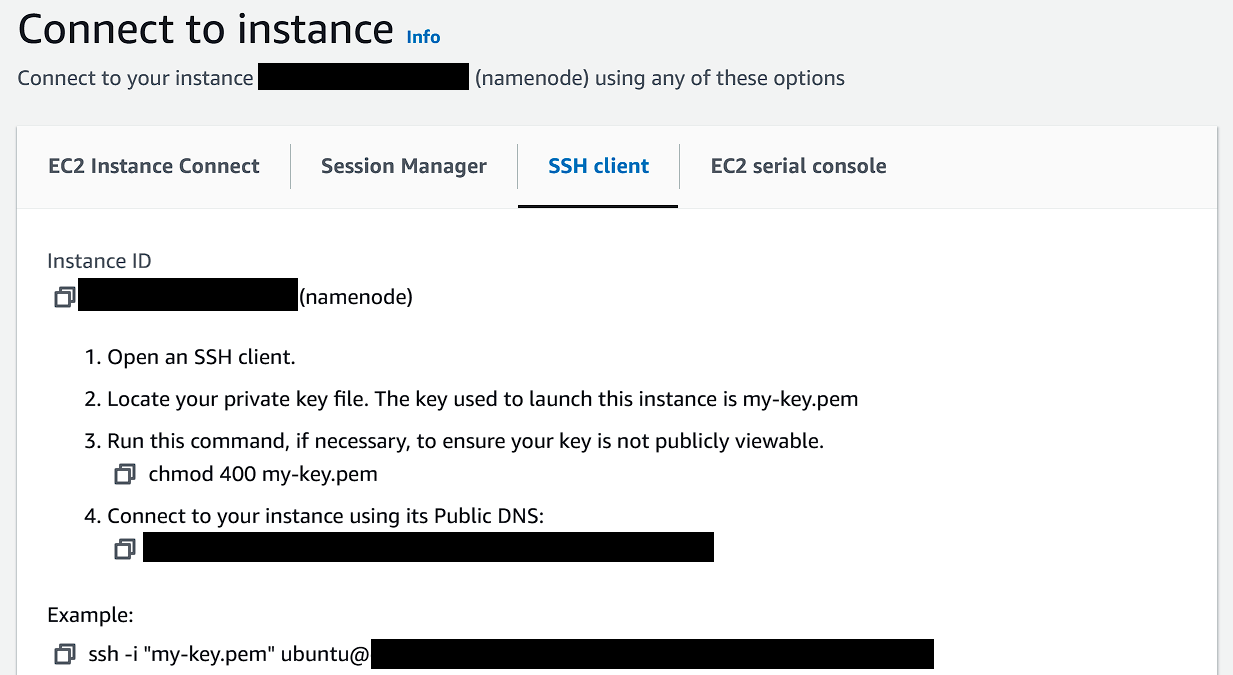
\includegraphics[width=0.7\textwidth]{images/instance-connect.png}
\end{figure}

Aprendo un terminale sul nostro computer potremo incollare il comando mostrato oppure digitarlo manualmente nel seguente modo (assicurandoci di essere nella cartella dove risiede il file della chiave, e con ADDRESS indichiamo l'indirizzo pubblico IPv4 che si può trovare nei dettagli dell'istanza selezionata):

\begin{verbatim}
    $ ssh -i my-key.pem ubuntu@ADDRESS
\end{verbatim}

Infine, per trasferire la chiave RSA nell'istanza master senza l'utilizzo di S3, possiamo utilizzare il seguente comando (con un secondo terminale e sempre dalla cartella in cui è presente la chiave):

\begin{verbatim}
    $ scp -i my-key.pem my-key.pem ubuntu@ADDRESS:/home/ubuntu/.ssh
\end{verbatim}

In questa maniera, in caso si dovesse perdere la chiave, si potrà accedere all'istanza dalla sezione \textbf{Ec2 Instance Connect} dello screenshot precedente (che permette di connettersi con un terminale web), e andando nella cartella \textbf{/home/ubuntu/.ssh} si ritroverà il file della chiave, che si potrà aprire con nano per recuperarne il contenuto e ri-salvarlo sul proprio computer come file .pem.
